\input{preamble_base}
\usepackage{makecell}
\newlength{\bibitemsep}\setlength{\bibitemsep}{.2\baselineskip plus .05\baselineskip minus .05\baselineskip}
\newlength{\bibparskip}\setlength{\bibparskip}{0pt}
\let\oldthebibliography\thebibliography
\renewcommand\thebibliography[1]{%
	\oldthebibliography{#1}%
	\setlength{\parskip}{\bibitemsep}%
	\setlength{\itemsep}{\bibparskip}%
}

\usepackage{tikz}


\begin{document}
	
\newcommand{\signfield}[2]{%
	\rule{#1}{0.1pt}\hspace{-#1}
	\raisebox{-1.1ex}{\parbox[t]{#1}{\centering\scriptsize{#2}}}
}

\thispagestyle{empty}
\begin{center}
	\large
	{\scshape министерство науки и высшего образования \\Российской Федерации}
	\vspace{1ex}
	
	{\scshape национальный исследовательский ядерный\\университет <<мифи>>}
	\vspace{2.5 cm}
	
	\large
	{\scshape \textbf{О\,Т\,Ч\,Е\,Т}\\о выполнении курсового проекта}
	{\scshape \textbf{<<теплогидравлический и нейтронно-физический расчет активной зоны реактора ВВЭР-1200>>}}
\end{center}

\vspace{2cm}
\begin{flushright}
	\textbf{Выполнил}\\студент группы С19-103\\
	Мамлеев А.\,А.\\[1ex]
	\signfield{3cm}{подпись}
\end{flushright}


\vspace{1 ex}
\parbox{0.5\linewidth}{
\begin{flushleft}
	\textbf{Научный руководитель\\по теплогидравлическому\\расчету}\\канд. техн. наук Маслов Ю.\,А.\\[1ex]
	\signfield{3cm}{подпись}
\end{flushleft}
}
\parbox{0.5\linewidth}{
\begin{flushleft}
	\textbf{Научный руководитель\\по нейтронно-физическому\\расчету}\\канд. физ.-мат. наук Савандер В.\,И.\\[1ex]
	\signfield{3cm}{подпись}
\end{flushleft}
}

\vspace{1 ex}
\textbf{Оценка (ECTS): }



\vfill

\begin{center}
	Москва 2024
\end{center}
\newpage


\textbf{Цель:} изучить методы синтеза комбинационных схем на логических элементах; получить навыки проектирования комбинационных схем на VHDL; овладеть инструментальными средствами проектирования схем на ПЛИС; приобрести опыт экспериментального исследования синтезируемых схем.

\section{Синтез комбинационной схемы}

В соответствии с вариантом дана следующая система ФАЛ:
\begin{equation} \label{eq: FAL}
	\left\{
	\begin{aligned}
		F_1(x_3, x_2, x_1, x_0) &= \sum(1, 3, 5, 7, 8, 10, 12, 14),\\
		F_2(x_3, x_2, x_1, x_0) &= \sum(1, 2, 3, 5, 7, 9, 15),\\
		F_3(x_3, x_2, x_1, x_0) &= \sum(1, 3, 5, 7, 8, 9).
	\end{aligned}
	\right.
\end{equation}

Для данных функций составим таблицу истинности (табл.~\ref{tab: true-false}).
\begin{table}[h]
	\centering
	\caption{Таблица истинности для системы ФАЛ \eqref{eq: FAL}} \label{tab: true-false}
	\begin{tabular}{|c||c|c|c|c||c|c|c|}
		\hline
		№ & $x_3$ & $x_2$ & $x_1$ & $x_0$ & $F_1$ & $F_2$ & $F_3$ \\
		\hline
		0 & 0 & 0 & 0 & 0 & 0 & 0 & 0 \\
		\hline
		1 & 0 & 0 & 0 & 1 & 1 & 1 & 1 \\
		\hline
		2 & 0 & 0 & 1 & 0 & 0 & 1 & 1 \\
		\hline
		3 & 0 & 0 & 1 & 1 & 1 & 1 & 1 \\
		\hline
		4 & 0 & 1 & 0 & 0 & 0 & 0 & 0 \\
		\hline
		5 & 0 & 1 & 0 & 1 & 1 & 1 & 1 \\
		\hline
		6 & 0 & 1 & 1 & 0 & 0 & 0 & 0 \\
		\hline
		7 & 0 & 1 & 1 & 1 & 1 & 1 & 1 \\
		\hline
		8 & 1 & 0 & 0 & 0 & 1 & 0 & 1 \\
		\hline
		9 & 1 & 0 & 0 & 1 & 0 & 1 & 1 \\
		\hline
		10 & 1 & 0 & 1 & 0 & 1 & 0 & 0 \\
		\hline
		11 & 1 & 0 & 1 & 1 & 0 & 0 & 0 \\
		\hline
		12 & 1 & 1 & 0 & 0 & 1 & 0 & 0 \\
		\hline
		13 & 1 & 1 & 0 & 1 & 0 & 0 & 0 \\
		\hline
		14 & 1 & 1 & 1 & 0 & 1 & 0 & 0 \\
		\hline
		15 & 1 & 1 & 1 & 1 & 0 & 1 & 0 \\
		\hline
	\end{tabular}
\end{table}

Произведем минимизацию функций методом диаграмм Вейча; на рис.~\ref{fig: diagram_sample} представлена эталонная диаграмма, которой далее будем пользоваться.
\begin{figure}
	\centering
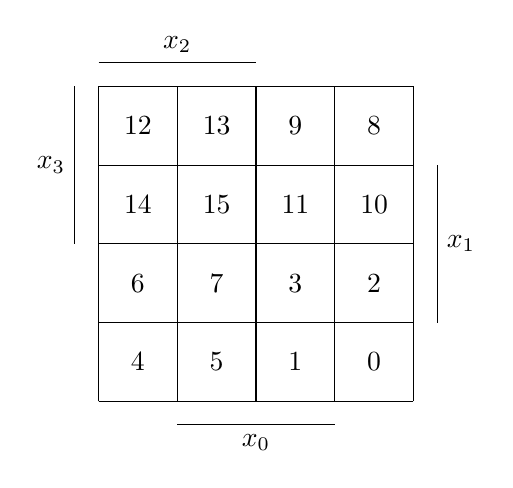
\begin{tikzpicture}
	\draw (0,0) grid (4,4);
	\node at (3.5, .5){0};
	\node at (2.5,.5){1};
	\node at (3.5, 1.5){2};
	\node at (2.5, 1.5){3};
	\node at (0.5, 0.5){4};
	\node at (1.5, .5){5};
	\node at (0.5, 1.5){6};
	\node at (1.5,1.5){7};
	\node at (3.5,3.5){8};
	\node at (2.5, 3.5){9};
	\node at (3.5, 2.5){10};
	\node at (2.5, 2.5){11};
	\node at (0.5, 3.5) {12};
	\node at (1.5,3.5){13};
	\node at (0.5, 2.5){14};
	\node at (1.5, 2.5){15};
	\draw (0,4.3) --node[midway, above]{$x_2$} (2,4.3);
	\draw (-0.3,4) --node[midway, left]{$x_3$} (-0.3,2);
	\draw (1,-0.3) --node[midway, below]{$x_0$} (3,-0.3);
	\draw (4.3,1) --node[midway, right]{$x_1$} (4.3,3);
\end{tikzpicture}
\caption{Эталонная диаграмма Вейча} \label{fig: diagram_sample}
\end{figure}

\begin{figure}[h]
	\captionsetup[subfigure]{justification=centerlast}
	\begin{subfigure}{0.3\linewidth}
		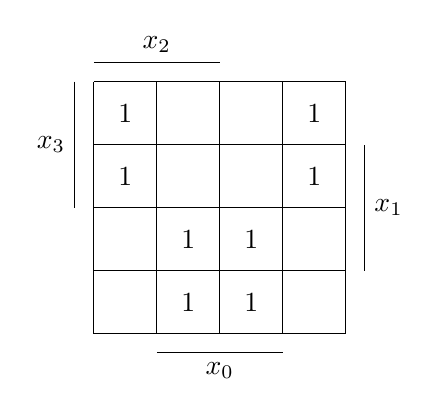
\begin{tikzpicture}[scale=0.8]
			\draw (0,0) grid (4,4);
			%\node at (3.5, .5){0};
			\node at (2.5,.5){1};
			%\node at (3.5, 1.5){2};
			\node at (2.5, 1.5){1};
			%\node at (0.5, 0.5){4};
			\node at (1.5, .5){1};
			%\node at (0.5, 1.5){6};
			\node at (1.5,1.5){1};
			\node at (3.5,3.5){1};
			%\node at (2.5, 3.5){9};
			\node at (3.5, 2.5){1};
			%\node at (2.5, 2.5){11};
			\node at (0.5, 3.5) {1};
			%\node at (1.5,3.5){13};
			\node at (0.5, 2.5){1};
			%\node at (1.5, 2.5){15};
			\draw (0,4.3) --node[midway, above]{$x_2$} (2,4.3);
			\draw (-0.3,4) --node[midway, left]{$x_3$} (-0.3,2);
			\draw (1,-0.3) --node[midway, below]{$x_0$} (3,-0.3);
			\draw (4.3,1) --node[midway, right]{$x_1$} (4.3,3);
		\end{tikzpicture}
		\caption{Для функции $F_1$} \label{fig:Veitch_F1}
	\end{subfigure}
	\hfill
	\begin{subfigure}{0.3\linewidth}
		\centering
		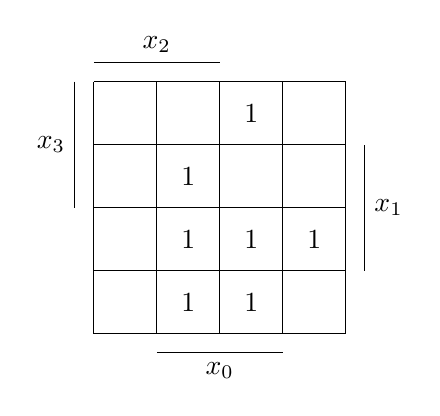
\begin{tikzpicture}[scale=0.8]
			\draw (0,0) grid (4,4);
			%\node at (3.5, .5){0};
			\node at (2.5,.5){1};
			\node at (3.5, 1.5){1};
			\node at (2.5, 1.5){1};
			%\node at (0.5, 0.5){4};
			\node at (1.5, .5){1};
			%\node at (0.5, 1.5){6};
			\node at (1.5,1.5){1};
			%\node at (3.5,3.5){8};
			\node at (2.5, 3.5){1};
			%\node at (3.5, 2.5){10};
			%\node at (2.5, 2.5){11};
			%\node at (0.5, 3.5) {12};
			%\node at (1.5,3.5){13};
			%\node at (0.5, 2.5){14};
			\node at (1.5, 2.5){1};
			\draw (0,4.3) --node[midway, above]{$x_2$} (2,4.3);
			\draw (-0.3,4) --node[midway, left]{$x_3$} (-0.3,2);
			\draw (1,-0.3) --node[midway, below]{$x_0$} (3,-0.3);
			\draw (4.3,1) --node[midway, right]{$x_1$} (4.3,3);
		\end{tikzpicture}
		\caption{Для функции $F_2$}\label{fig:Veitch_F2}
	\end{subfigure}
	\hfill
	\begin{subfigure}{0.3\linewidth}
		\centering
		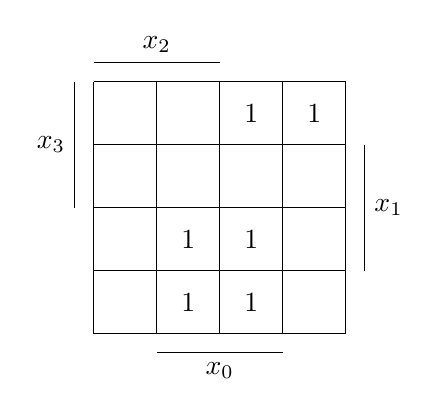
\begin{tikzpicture}[scale=0.8]
			\draw (0,0) grid (4,4);
			%\node at (3.5, .5){0};
			\node at (2.5,.5){1};
			%\node at (3.5, 1.5){2};
			\node at (2.5, 1.5){1};
			%\node at (0.5, 0.5){4};
			\node at (1.5, .5){1};
			%\node at (0.5, 1.5){6};
			\node at (1.5,1.5){1};
			\node at (3.5,3.5){1};
			\node at (2.5, 3.5){1};
			%\node at (3.5, 2.5){10};
			%\node at (2.5, 2.5){11};
			%\node at (0.5, 3.5) {12};
			%\node at (1.5,3.5){13};
			%\node at (0.5, 2.5){14};
			%\node at (1.5, 2.5){15};
			\draw (0,4.3) --node[midway, above]{$x_2$} (2,4.3);
			\draw (-0.3,4) --node[midway, left]{$x_3$} (-0.3,2);
			\draw (1,-0.3) --node[midway, below]{$x_0$} (3,-0.3);
			\draw (4.3,1) --node[midway, right]{$x_1$} (4.3,3);
		\end{tikzpicture}
		\caption{Для функции $F_3$}\label{fig:Veitch_F3}
	\end{subfigure}
	\caption{Диаграммы Вейча для заданных функций}\label{fig:Veitch_all}
\end{figure}

Произведя минимизацию при помощи диаграмм Вейча (рис.~\ref{fig:Veitch_all}), запишем заданные функции в форме МДНФ:
\begin{equation}
	\left\{
	\begin{aligned}
		F_1(x_3, x_2, x_1, x_0) &= x_0\bar x_3 \vee \bar x_0 x_3,\\
		F_2(x_3, x_2, x_1, x_0) &= x_0\bar x_3 \vee x_0 x_1 x_2 \vee x_0\bar x_1 \bar x_2 \vee x_1\bar x_2\bar x_3,\\
		F_3(x_3, x_2, x_1, x_0) &= x_0\bar x_3 \vee \bar x_1\bar x_2 x_3.
	\end{aligned}
	\right.
\end{equation}

\section{Описание комбинационной схемы на VHDL}

\end{document}